\begin{figure}[htbp]
    \centering
    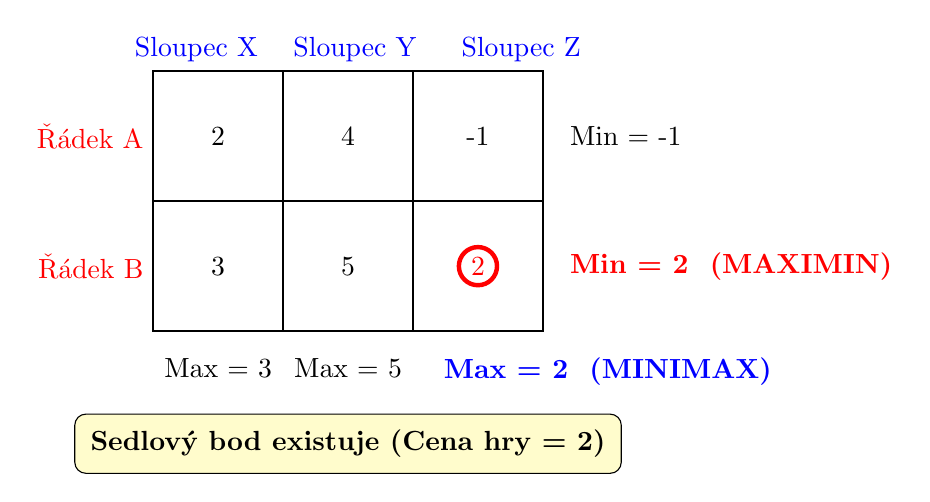
\begin{tikzpicture}[scale=1.1]
        % Mřížka matice 2x3
        \draw[thick] (0,0) rectangle (4.5, 3);
        \draw[thick] (1.5,0) -- (1.5,3);
        \draw[thick] (3,0) -- (3,3);
        \draw[thick] (0,1.5) -- (4.5,1.5);

        % Hlavičky řádků a sloupců
        \node[red, left] at (0, 2.25) {Řádek A};
        \node[red, left] at (0, 0.75) {Řádek B};
        \node[blue, above] at (0.5, 3) {Sloupec X};
        \node[blue, above] at (2.33, 3) {Sloupec Y};
        \node[blue, above] at (4.25, 3) {Sloupec Z};

        % Hodnoty v buňkách (Výplata pro Řádkového hráče)
        \node at (0.75, 2.25) {2};
        \node at (2.25, 2.25) {4};
        \node at (3.75, 2.25) {-1};

        \node at (0.75, 0.75) {3};
        \node at (2.25, 0.75) {5};
        % Sedlový bod zakroužkujeme
        \node[draw, circle, red, ultra thick, inner sep=2pt] at (3.75, 0.75) {2}; 

        % Nalezení řádkových minim
        \node[right] at (4.7, 2.25) {Min = -1};
        \node[right, red, font=\bfseries] at (4.7, 0.75) {Min = 2 \ (MAXIMIN)};

        % Nalezení sloupcových maxim
        \node[below] at (0.75, -0.2) {Max = 3};
        \node[below] at (2.25, -0.2) {Max = 5};
        \node[below, blue, font=\bfseries] at (5.25, -0.2) {Max = 2 \ (MINIMAX)};

        % Závěr
        \node[align=center, font=\bfseries, fill=yellow!20, draw, rounded corners, inner sep=2mm] 
        at (2.25, -1.3) {Sedlový bod existuje (Cena hry = 2)};
    \end{tikzpicture}
    \caption{Řešení hry s nulovým součtem. Maximin řádkového hráče je roven Minimaxu sloupcového hráče, hra má tedy čisté řešení.}
\end{figure}